% Este arquivo .tex será incluído no arquivo .tex principal. Não é preciso
% declarar nenhum cabeçalho

\section{Eventos da Unicamp}
\subsection{Feira do Livro}

Evento iniciado em 2002, a cada dois anos a Editora da Unicamp realiza a Feira
do Livro, no Ginásio da Unicamp. Há excelentes opções, de diversas editoras,
principalmente na área de literatura, artes e humanas, com no mínimo 50\% de
desconto.

\subsection{Semanas da Unicamp}

Alguns cursos da Unicamp realizam anualmente um evento (chamado de Semana) em
que os alunos de graduação têm um contato com o mercado de trabalho, com as
pesquisas, com as tendências e novidades dos cursos e demais assuntos, ramos e
áreas de cada curso. Para isso, participam desse evento ex-alunos e
profissionais, realizam-se palestras e minicursos, são feitas visitas a empresas
e são feitos debates (mesas redondas).

\subsubsection*{Secomp -- Semana da Computação}

\begin{figure}[H]
    \centering
    
\includegraphics[scale=0.20]{img/alem_da_graduacao/secomp_logo.png}
\end{figure}

A Computação tem a sua própria semana, organizada por três entidades estudantis:
CACo, AAACEC e Conpec. O evento busca aproximar e relacionar os três pilares da
graduação: os alunos, a universidade e o mercado. Dessa forma, a Secomp --
Semana da Computação -- procura mostrar aos alunos a diversidade de caminhos a
seguir e um pouco do que cada área pode oferecer.

Durante seus sete dias de duração, a Semana traz uma gama de atividades, entre
palestras, oficinas, cursos, visitações e outros eventos, para que os
participantes possam ter uma visão abrangente do mercado e da própria
universidade. Além disso, a Secomp tem atividades voltadas ao recrutamento em
grandes empresas, para aqueles à procura de vagas.

Se você acha que nada disso importa, bixo, você é burro, mas não tem problema.
A Semana também tem uma fartura -- literalmente -- de coffee-breaks, brindes e
prêmios sorteados. Tudo isso por um preço simbólico, menor do que o de uma
balada no Campinas Hall. Não perca!

\subsection{Talento}

Talento é um evento que acontece todo ano, desde 1999, durante um dia inteiro,
no Ginásio Multidisciplinar e organizado pelo Núcleo de Empresas Juniores da
Unicamp. Trata-se de uma feira de recrutamento, onde alunos da Unicamp e de
outras universidades e o público em geral têm contato com empresas, seja por
meio de palestras, mesas redondas e estandes, e estas apresentam o seu processo
seletivo. Nesse evento também é feito o cadastro de currículos dos visitantes.

Para saber mais sobre o evento, é só acessar a página da Talento
(\url{talentounicamp.com.br}). O evento é gratuito.

\subsection{UPA -- Unicamp de Portas Abertas}

\begin{figure}[h!]
    \centering
    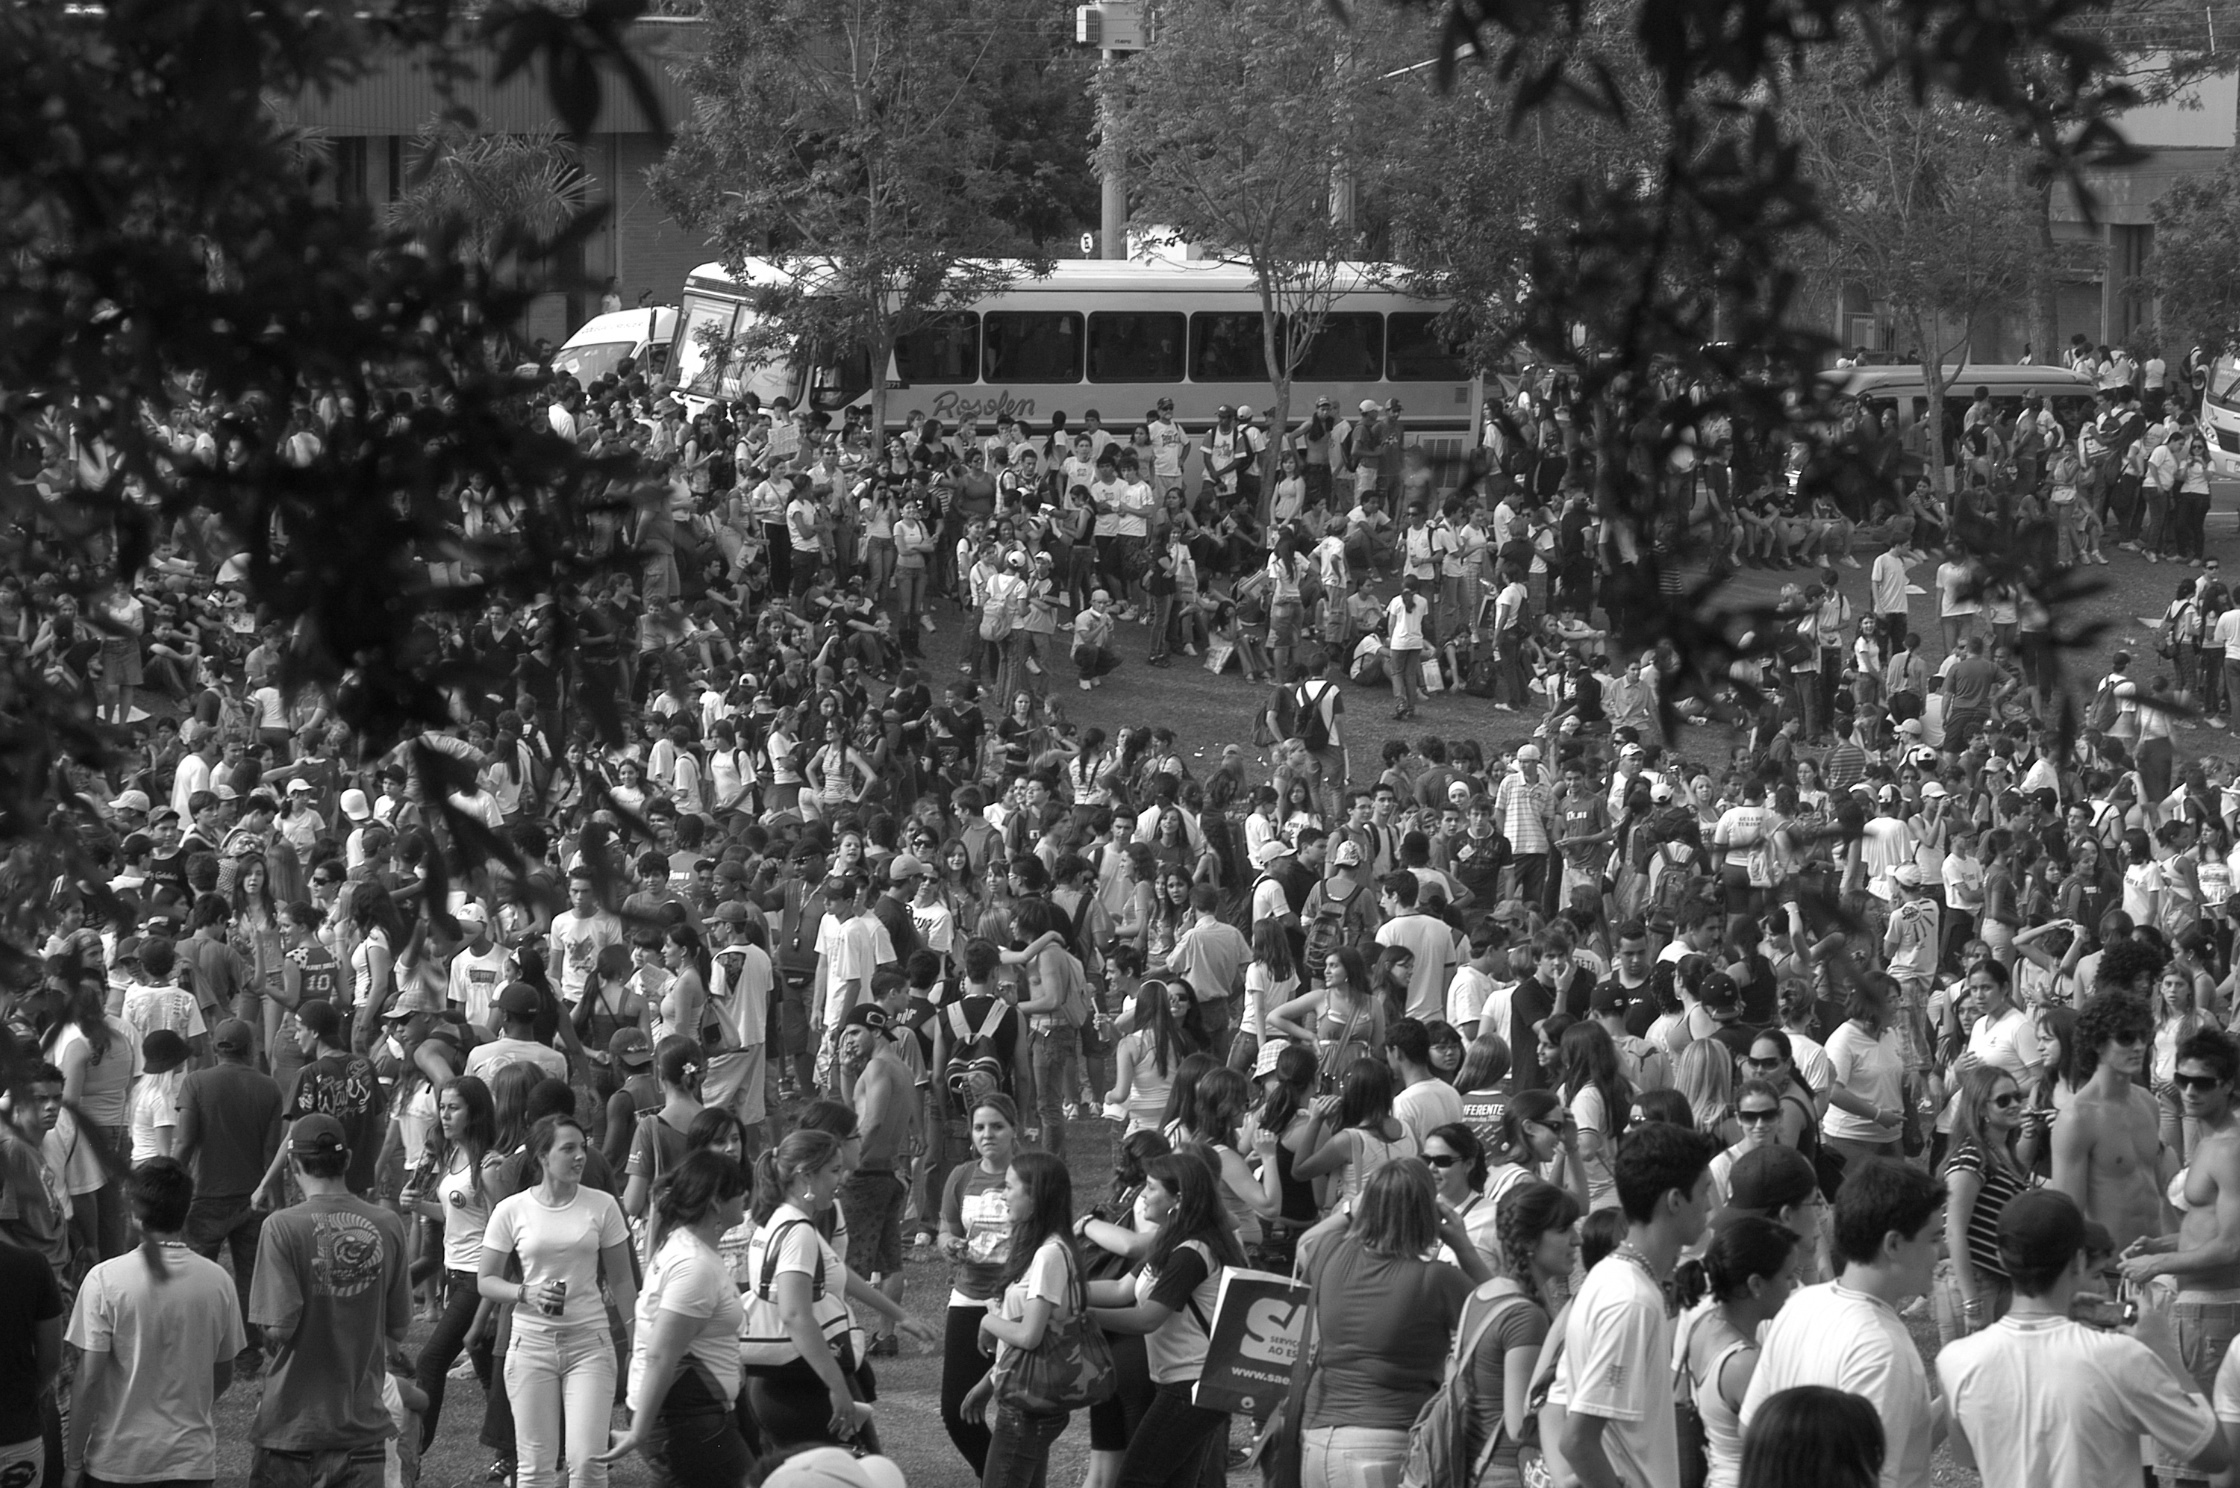
\includegraphics[scale=0.38, keepaspectratio=true]{img/imgs/bateria.jpg}
\end{figure}

A \textbf{UPA} é um evento anual em que, durante um dia, geralmente no mês de
setembro, a Unicamp é apresentada para estudantes dos ensinos fundamental e
médio de todo o país, muitos dos quais pré-vestibulandos. A apresentação da
universidade é feita por professores e alunos, que mostram as salas de aula e as
pesquisas realizadas.

No ano de 2013, a UPA recebeu a visita de 40 mil alunos de 639 escolas públicas
e privadas, originárias de vários estados do Brasil.

O IC costuma realizar uma recepção com forte participação dos alunos. Se você é
como todo bixo e está louco para pagar de estudante da Unicamp, esta é uma
oportunidade excelente! Além de ser divertido, o IC geralmente oferece uma
pequena remuneração pelo trabalho. Participe!

Para saber mais sobre o evento, é só acessar a página \url{www.upa.unicamp.br}.
